\documentclass{beamer}

% Choose a built-in theme
\usetheme{Copenhagen}
\usecolortheme{beaver}
\usepackage{listings}
% SVG figures are converted to PDF by latexmk (see latexmkrc)
\DeclareGraphicsExtensions{.pdf,.png,.jpg}
% Scale a figure to fit the remaining slide space, keeping its aspect ratio
\newcommand{\slidefig}[1]{\includegraphics[width=\linewidth,height=0.6\textheight,keepaspectratio]{#1}}

\lstset{
  breaklines=true
}

\title{A complexity analysis of loopy}
\author{Tom Griffiths}

\begin{document}

% Title Slide
\begin{frame}
    \titlepage
\end{frame}

% Content Slide
\begin{frame}{What is loopy?}
    \begin{itemize}
        \item Played on a planar graph
        \item Objective is to find a loop without self-intersection
        \item Numbered faces must have exactly n edges in the path
        \item A unique solution exists
    \end{itemize}
\end{frame}

\begin{frame}{Is loopy NP-complete?}
    \begin{enumerate}
        \item Is there a polynomial-time way to a verify a solution? (in NP)
        \item Can we reduce it another NP-complete problem to loopy in polynomial time? (NP-Hard)
    \end{enumerate}
\end{frame}

\begin{frame}{Is loopy in NP?}
    This is trivial
    \lstinputlisting[firstline=33, lastline=57,basicstyle=\ttfamily\tiny]{../game/src/loopy.ts}
\end{frame}

\begin{frame}{What is a reduction?}
    Let $f::\alpha \rightarrow Boolean$ solve decision problem $\alpha$ correctly and $g::\beta \rightarrow Boolean$ solve decision problem $\beta$ correctly. \\
    A (turing) reduction from $\alpha$ to $\beta$ is a function $h\ g$ with $h::(\beta \rightarrow Boolean) \rightarrow \alpha \rightarrow Boolean$. \footnotemark \\
    Then \\
    $\exists h\forall f\forall g\ s.t.\ O(h)\subseteq O(f\ g)$.
    \footnotetext{This is a non-standard definition but it uses functional programming which is cool}
\end{frame}

\begin{frame}{Recap of CNF-SAT}
    A CNF SAT instance is a set of clauses, where each clause is a disjunction of literals. \\
    A solution is a truth assignment to each literal that satisfies all clauses.
    $$(x\lor y\lor z)\land (x\lor \neg z)\land (\neg x\lor y\lor \neg z)$$
    In this case one such solution is $(x, y, z) = (T, T, F)$.
\end{frame}

\begin{frame}{The reduction}
    We want to construct gadgets that respresent properties of the CNF SAT problem.
    \begin{itemize}
        \item Each clause must have at least one true literal
        \item For a variable $x$ exactly one of $x$ and $\neg x$ must be true
    \end{itemize}
    We will represent true by the presence of the loopy line.
\end{frame}

\begin{frame}{The clause gadget}
    The clause gadget is a polygon where exactly one edge must be saturated. Two edges between each literal prevents cross over from other variables.
    \begin{figure}
        \centering
        \slidefig{images/clause_gadget}
    \end{figure}
\end{frame}

\begin{frame}{The variable gadget}
    The variable gadget involves a diverging branch where only one side can be saturated.
    \begin{figure}
        \centering
        \slidefig{images/variable_gadget}
    \end{figure}
\end{frame}

\begin{frame}{Implementation in polynomial time}
    \lstinputlisting[firstline=10, lastline=23,basicstyle=\ttfamily\tiny]{../backend/loopy.py}
\end{frame}

\begin{frame}{Implementation in polynomial time}
    \lstinputlisting[firstline=25, lastline=39,basicstyle=\ttfamily\tiny]{../backend/loopy.py}
\end{frame}

\begin{frame}{Implementation in polynomial time}
    \lstinputlisting[firstline=44, lastline=61,basicstyle=\ttfamily\tiny]{../backend/loopy.py}
\end{frame}

\begin{frame}{Conclusion?}
    We have shown that the CNF SAT can be reduced to loopy and hence loopy is NP-complete.
    Let's see what this looks like in practice. \\
    We will use the Fruchterman-Reingold algorithm to display the graph on a plane.
    \lstinputlisting[firstline=25, lastline=42,basicstyle=\ttfamily\tiny]{../backend/arrangement.py}
\end{frame}

\begin{frame}{3D}
    \begin{figure}
        \centering
        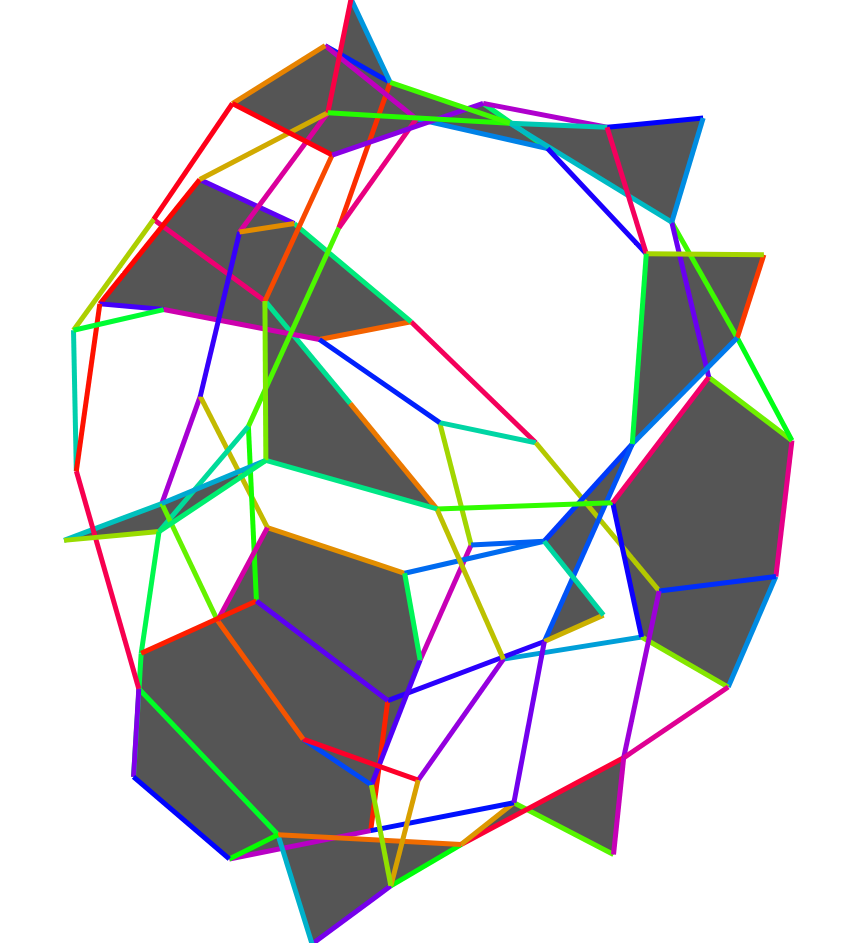
\includegraphics[height=3in]{2d_loopy.png}
    \end{figure}
\end{frame}

\begin{frame}{3D}
    \begin{figure}
        This is very hard to understand let's put it into 3D to get a better idea of the situation.\\
        \begin{itemize}
            \item WebGL rendering
            \item Add one more dimension
            \item Cloudflare hosting
            \item https://loopy.noon-tech.co.uk
        \end{itemize}
    \end{figure}
\end{frame}

\begin{frame}{3D}
    % \begin{figure}
    %     \centering
    %     \includegraphics[height=3in]{3d_loopy.png}
    %     \caption{}
    % \end{figure}
\end{frame}

\begin{frame}{Problems}
    We have currently ignored the planarity requirement and the uniqueness requirements. These restrictions could possibly unlock new solving strategies and may comprise our NP-Completeness.
\end{frame}

\begin{frame}{Uniqueness}
    Uniqueness is a useful constraint to have when solving by hand
    \begin{figure}
        \centering
        \slidefig{images/uniqueness_counterexample}
    \end{figure}
\end{frame}

\begin{frame}{Uniqueness}
    This is constraint is somewhat tricky to formally phrase. We are not checking uniqueness we are assuming it. Let $A(x)$ denote the number of a solution to the problem for an instance $x$ then for some predicate $Q(x)$ the result of algorithm is $U(x)$ where
    $$U(x)=\begin{cases}
        A(x)=0 & 0 \\
        A(x)=1 & 1 \\
        A(x)>1 & Q(x)
    \end{cases}$$
    % Now we are able to define our algorithm on the whole domain
\end{frame}

\begin{frame}{Uniqueness}
    To show uniqueness we need a reduction from a problem that is NP-hard when uniqueness is promised. Additionally the reduction should be parsimonious. This means it preserves the number of solutions to the problem.
\end{frame}

\begin{frame}{Is 3-USAT NP-Complete}
    Let us consider 3-USAT which is 3-SAT where there is promised to at most one satisifying assignment. \\
    It is easy to see 3-USAT$\in$NP but it remains to show that it is still NP-Hard.\footnotemark
    \footnotetext{I've always wanted to say this}
\end{frame}

\begin{frame}{Valiant–Vazirani theorem}
    The Valiant–Vazirani theorem states that if 3-USAT$\in$P then $RP=NP$. Using proof by popular consensus $RP\neq NP$ hence 3-USAT is NP-complete.
    % Might prove this
\end{frame}

\begin{frame}{Is the reduction parsimonious}
    Our current reduction is not parsimonious. Consider $(x_1\lor x_2)\land (x_1\lor \lnot x_2) \land (\lnot x_1\lor x_2)$.
    \begin{figure}
        \centering
        \slidefig{images/non_unique}
    \end{figure}
\end{frame}

\begin{frame}{Making it parsimonious}
    For 2 variables the following structure can model an or.
    \begin{figure}
        \centering
        \slidefig{images/2-or-unique}
    \end{figure}
\end{frame}

\begin{frame}{Making it parsimonious}
    We can naively expand this to 3 variables but this is not unique for the case (0,1,1)
    \begin{figure}
        \centering
        \slidefig{images/naive-3-or}
    \end{figure}
\end{frame}

\begin{frame}{Making it parsimonious}
    We can deal with this by enforcing an extra restriction and adding this always on line for cases (1,0,0) and (0,1,0).
    \begin{figure}
        \centering
        \slidefig{images/true-3-or}
    \end{figure}
    This device completes our reduction but is not planar.
\end{frame}

\begin{frame}{Planarity}
    This constraint is more formally topologically equilivant to a sphere. This is a useful constraint to have e.g. in the four colour theorem. Additionally there is an idea for an improved solver in the loopy code that relies on it.
    \lstinputlisting[firstline=15, lastline=27,basicstyle=\ttfamily\tiny]{./loopy.c}
     \footnotetext{Obviously I mean the 2-sphere}
\end{frame}

\begin{frame}{How to ensure planarity}
    We already have a weaker condition whereby no edge is connected to more than two faces. This means all that would be left is constructing a gadget that can be used to replace two crossing edges. Such a structure exists but it raises a lot of problems
    \begin{itemize}
        \item How to ensure this doesn't split the loop
        \item Does this preserve uniqueness of solutions
        \item Is the number of crossing points polynomial
    \end{itemize}
\end{frame}

\begin{frame}{Why we won't be considering planarity}
    \begin{itemize}
        \item The questions are difficult and annoying to reason about.
        \item I would have written a 3d version for no reason
        \item I don't want to overun massively
        \item Playing loopy on different topological shapes would be cool
    \end{itemize}
\end{frame}

\end{document}
